\section{Method}
Both the spectrums and the images will be analysed using spectrometer methods, this will open up for the opportunity to pre-process spectral and spatial data in the same way. We will then hopefully be able to compare the data more directly. The spectrometer processing method we want to use is relative reflectance ($RR$). Since this method is also being used with the spectrometer, it will be denoted $RR'$ whenever it is used for imaging. As can be seen from (\ref{eq:relative_reflectance}), relative reflectance is done by dividing the interesting values with a reference. The translation to image processing must be to divide every image pixel with a pixel value from a reference image. For comparing values with the spectrometer it is fully ok to do this division as long as the reference image is non-zero for all pixels. For that reason it is important with a well lit and preferably white background. 


One problem with this method is that images can only be visualized as three sets of integers between 0 and 255, i.e. the colors blue, green and red. Therefore we divide the division into to two cases when visualizing; reference divided by image and image divided by reference. We will denote the product $RR'_{negative}$ for the reference divided by image case, and $RR'_{positive}$ for the image divided by reference case. The processing can be view in figure \ref{fig:image_visualization_program_flow} 

\begin{figure}[h]
    \centering
    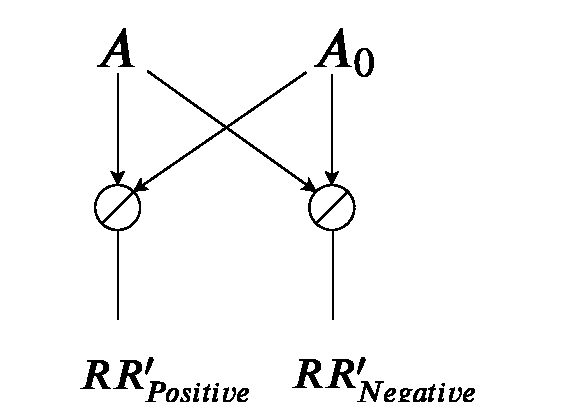
\includegraphics[width=0.5\textwidth]{figures/image_program_flow.pdf}
    \caption{Image visualization process flow}
    \label{fig:image_visualization_program_flow}
\end{figure}


\subsection{Spectrum processing}
\label{sec:spectrum_processing}

\begin{figure}[h]
    \centering
    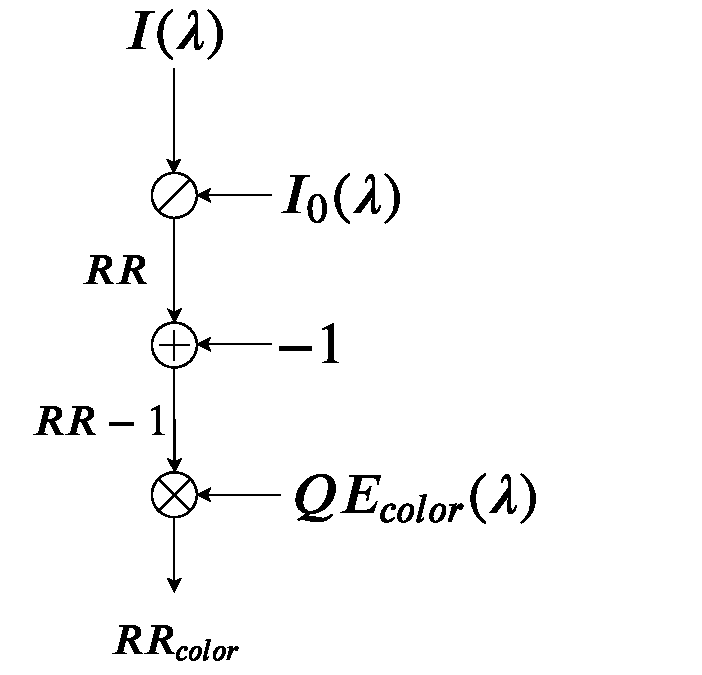
\includegraphics[width=0.5\textwidth]{figures/thesis_program_flow.pdf}
    \caption{Spectrum process flow}
    \label{fig:spectrum_process_flow}
\end{figure}

\subsection{Correlating Spectrometer to Camera}
\label{sec:method_correlating_spectrum_to_camera}
To get an idea of how well calibrated the camera is to the spectrometer and vice versa I propose the following calculation: 
Take the spatial average across the image from the camera and divide it with the spectral average of the spectrometer. 

\begin{equation}
    \label{eq:correlating_spectrum_to_camera}
    K = \frac{\mean{\vec{p}}}{\mean{RR}}
\end{equation}

This process is shown in figure \ref{fig:correlating_spectrum_and_image}.

\begin{figure}[h]
    \centering
    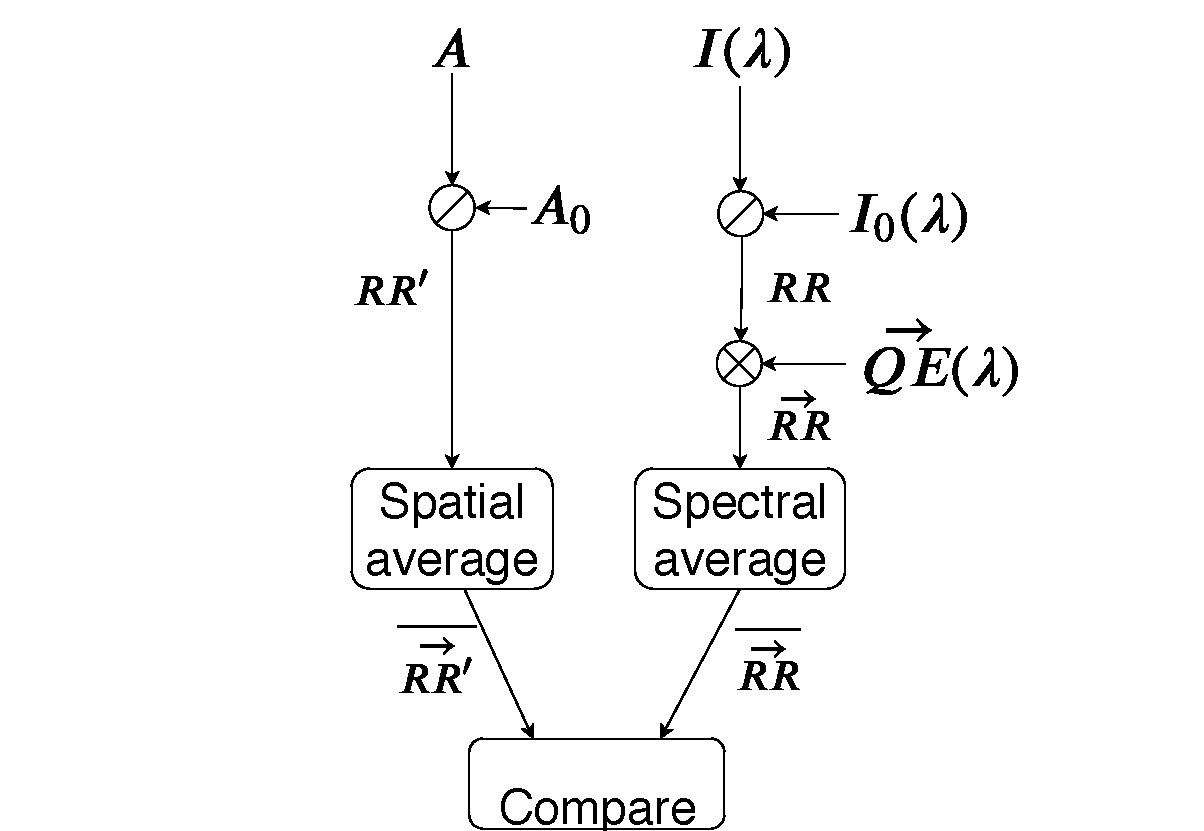
\includegraphics[width=0.75\textwidth]{figures/image_comparison_with_spectrometer.pdf}
    \caption{Correlating value between image and spectrum}
    \label{fig:correlating_spectrum_and_image}
\end{figure}


\subsection{Light}
Light is a crucial part of this project, as it is the source of input for both the camera and the spectrometer. It's also the link between the two sensors. The choosing of a sensor that can support both sensor types is therefore paramount. The camera is less selective on the spectral properties of the light source as it only requires a light source that is approximately white, i.e. have similar amounts of red, green and blue "wavelengths". It is however more selective in the spatial region as it can arise more problems for the camera if the lighting creates a lot of shadows or local problems like strong specular reflection making the pixel go into saturation. As implied the spectral properties of the light is more important for the spectrometer. For the spectrometer we want the spectrum to be as flat as possible. 

The characterization of the light source will be based on considerations from \cite{martinPracticalGuideMachine}, but also unfortunately be limited by available sources at the lab. % This paper provides a longer checklist, that can be simplified greatly under the following conditions: Stationary objects,
